\section{Schlussfolgerung}

Aus den soeben diskutierten Daten über das Material kann man folgende Erkenntnisse ableiten. Aus der Elektronenmobilität bei Raumtemperatur von
$$\mu=4961(13) \unit{\square\cm\per\V\per\s}$$

lässt sich ableiten, dass diese wesentlich größer ist als die von Silizium und Germanium (vgl. \cite{Halbleiterwerkstoffe}). Der ermittelte Wert liegt bei einem für n-dotiertes Galliumarsenid typischen Wert (vgl. \cite{GaAsWaverDaten}). Bei Betrachtung der Ionisierungsenergie von $E_d=0.0091(4) \unit{eV}$ und der Literaturwerte in Abbildung \ref{fig:ePlotIonisierungsenergien} stellt man fest, dass diese zwischen den typischen Werten für schwefel- und tellurdotiertem Galliumarsenid liegt (vgl. \cite{sPhysikHalbleiterBautauelemnte}). Somit lässt sich über das genaue Dotierungsverhalten keine Aussage treffen.
\\
\begin{figure}
    \centering
    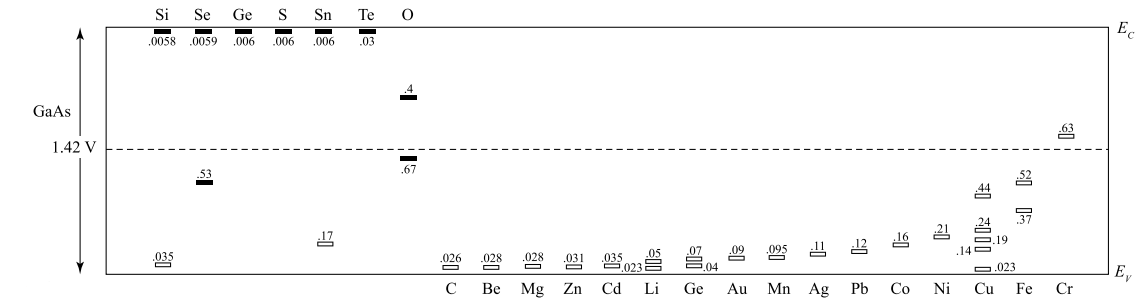
\includegraphics[width=\linewidth]{bilder/PlottIonisierungsenergien.png}
    \caption{
In dieser Abbildung sind gemessene Ionisierungsenergien für Galliumarsenid angegeben. Dabei sind die ausgefüllten Kästchen Donatorniveaus und die leeren Akzeptorniveaus \cite{sPhysikHalbleiterBautauelemnte}. }
    \label{fig:ePlotIonisierungsenergien}
\end{figure}



Weiters lässt sich bei der Betrachtung der Streuprozesse eine Unterteilung in 3 Mechanismen beobachten. Diese wäre Ionisierte Stoßstellen bei tiefen Remperaturen, Interaktion mit Phononen bei hohen Temperaturen, sowie einen Bereich bei dem diese zwei Mechanismen mischen. Wo lässt sich nun die Matthiessensche Regel beobachten?
Sie äußert sich an den Steigungen der beiden Bereiche im doppelt logarithmischen Plot, welche im Rahmen ihrer Unsicherheit mit $\pm 3/2$ nicht vertragbar sind, wobei $a = \pm 3/2$ die Steigung bei rein phononischer bzw. ionischer Streuung darstellt. Kurz gesagt, selbst in den Nieder- und Hochtemperaturbereichen gibt es immer eine Mischung der Streumechanismen.
\\


Wie könnte der Versuch verbessert werden? Die wohl signifikanteste Verbesserung würde durch eine automatische, gleichzeitige Erfassung aller gemessenen Größen erreicht werden. Eine weitere Verbesserung wäre die Verwendung eines Tieftemperatursensors, da der PT100 bei sehr niedrigen Temperaturen an seine Grenzen stößt.
\\



Im Großen und Ganzen ist es somit gelungen, durch die van-der-Pauw-Methode mit unspektakulären Spannungsmessungen sowie einer Temperaturmessung fundamentale Eigenschaften wie Dotierung und Material, aber auch anwendungsnahe Größen wie Leitwerte und deren Verhalten zu bestimmen. Damit reiht sich dieser Versuch in eine Serie von Experimenten ein, bei denen die ausgeklügelte Anwendung der Theorie zu einem gut durchführbaren Experiment führt, dessen Erkenntnisse jedoch angesichts seiner geringen Komplexität geradezu überraschend sind. Dies unterstreicht die Effizienz solcher praxisnahen Ansätze und zeigt, dass auch mit vergleichsweise einfachen Methoden tiefgreifende Einblicke in die Materie gewonnen werden können.
